\documentclass[conference]{IEEEtran}
\usepackage[T1]{fontenc}
\IEEEoverridecommandlockouts
% The preceding line is only needed to identify funding in the first footnote. If that is unneeded, please comment it out.
\usepackage{cite}
\usepackage{amsmath,amssymb,amsfonts}

\usepackage[linesnumbered,ruled,vlined]{algorithm2e}
\DontPrintSemicolon
\usepackage[hidelinks]{hyperref}
\usepackage[noabbrev,capitalize]{cleveref}
\usepackage{array, booktabs, makecell}
\usepackage{graphicx}
\usepackage{textcomp}
\usepackage{xcolor}
\usepackage{caption}
\usepackage{subcaption}

\usepackage{tikz}
\usetikzlibrary{trees}

\newcommand\norm[1]{\left\lVert#1\right\rVert}
\def\BibTeX{{\rm B\kern-.05em{\sc i\kern-.025em b}\kern-.08em
    T\kern-.1667em\lower.7ex\hbox{E}\kern-.125emX}}

\graphicspath{../}
\hypersetup{
    colorlinks=true,
    linkcolor=black,
    filecolor=black,      
    citecolor=black,
    urlcolor=blue,
    pdfpagemode=FullScreen,
    }

\begin{document}

\title{Parallel Huffman Coding}

\author{\IEEEauthorblockN{Francesco Bozzo}
    \IEEEauthorblockA{\textit{DISI, University of Trento} \\
        Trento, Italy\\
        francesco.bozzo@studenti.unitn.it\\
        229312}
    \and
    \IEEEauthorblockN{Michele Yin}
    \IEEEauthorblockA{\textit{DISI, University of Trento} \\
        Trento, Italy\\
        michele.yin@studenti.unitn.it\\
        229359}
}

\maketitle

% add page number
\thispagestyle{plain}
\pagestyle{plain}

\begin{abstract}
    This report aims to explain the design of a parallel encoding and decoding Huffman algorithm. The application is developed with the C99 programming language, using MPI for multiprocessing and OpenMP for multithreading to scale horizontally with increasing hardware resources. Our tool is both able to exploit multiprocessing to process concurrently multiple folders, and to split the Huffman coding of the same file among multiple threads.

    Comparing this tool with other online implementations, we can state that\dots
\end{abstract}

\begin{IEEEkeywords}
    Huffman, MPI, OpenMP, High Performance Computing
\end{IEEEkeywords}

\section{Introduction}
The \emph{Huffman algorithm} is designed to find a more convenient bit representation, to store data through lossless compression. Instead of considering groups of eight bits to encode data, the Huffman algorithm uses variable length sequences of bits defined as \emph{alphabet}.

The objective of our work is to build a scalable Huffman encoder and decoder that are able to scale according to the provided hardware resources. Moreover, the application should handle both single files and nested folders properly.

Even if nowadays the Huffman algorithm is mainly used for teaching purposes, its prefix mechanism is still part of many notable standards, such as Deflate (PKZIP's algorithm), JPEG, and MP3 compression algorithms. For this reason, there are no state-of-the-art online-available implementations to compare our tool with. In fact, differently from our work, many of the tools we found are not built considering low-level optimizations (such as to use in-memory buffers to improve I/O timings) or non-essential features (such as folders and big files handling).

\section{The Huffman algorithm}
The Huffman algorithm has the objective of finding a more convenient bit representation to store information through lossless compression. Instead of considering groups of eight bits as the way to encode data, the Huffman algorithm uses variable-length sequences of bits with prefixes defined as \emph{alphabet}.

\subsection{Priority Queue}
The Huffman algorithm uses a minimum priority queue to build its alphabet efficiently. This specific data structure ensures logarithmic insertion and deletion time with respect to its size.
We implemented the minimum priority queue by using a minimum heap. Practically speaking, to implement the min-heap tree, we used a standard C array ensuring that the min-heap property still holds at every insertion and deletion:
\begin{equation}
    A[i] \le A[l(i)], A[i] \le A[r(i)]
\end{equation}
where \(A[i]\), \(A[l(i)]\), \(and A[r(i)]\) are respectively a node, its left child, and its right child in a min-heap tree.

To implement the priority queue also a parallel approach has been considered \cite{BRODAL19984}, but since it contains only 256 elements (1 byte), we did not consider it too important in terms of performance.

\subsection{Encoding}
The Huffman encoding procedure makes use of a minimum priority queue to build its alphabet efficiently. The idea is to build a tree similar to \cref{fig:tree} that defines all the variable-length prefix sequences of bits: these sequences are represented by the path from the tree root to a leaf. Using a greedy approach, the Huffman encoding ensures that the less frequent a byte is in a file, the more probable is to have a longer Huffman representation, which means that his path from the root to its specific leaf is longer.

Once having computed the frequencies for each one of the 256 different bytes in a file, the Huffman algorithm populates a min priority queue with Huffman tree nodes storing the byte value and its frequency. Successively, it removes the least two frequent bytes from the queue, creates a new node with children the two extracted nodes, assigns to it a dummy character and the sum of the frequencies of its two children, and inserts it into the min priority queue. After \(n-1\) iterations, the last node is the root of the Huffman tree \cite{bertossi2010algoritmi}. \Cref{alg:buildtree} explains in the detail this procedure.
\begin{algorithm}
    \caption{Build the Huffman tree}\label{alg:buildtree}

    \SetKwData{Q}{Q}\SetKwData{z1}{z1}\SetKwData{z2}{z2}\SetKwData{z}{z}
    \SetKwFunction{insert}{insert}\SetKwFunction{deleteMin}{deleteMin}
    \SetKwInOut{Input}{input}\SetKwInOut{Output}{output}
    \SetKwFor{}{}{}{}

    // Populate the min priority queue with characters and their frequencies\;
    \For{\(i=1\) \KwTo \(n-1\)}{
        Q.insert(f[i], Tree(f[i], c[i]))\;
    }
    // Repeat until the queue has only a single element left\;
    \For{\(i=1\) \KwTo \(n-1\)}{
        // Get the two least frequent nodes\;
        z1 = Q.deleteMin()\;
        z2 = Q.deleteMin()\;

        // Create an inner tree node and insert it into the queue\;
        z = Tree(z1.f + z2.f, null)\;
        z.left = z1\;
        z.right = z2\;
        Q.insert(z.f, z)\;
    }

    // The last element in the queue is the root of the Huffman tree\;
    \Return{Q.deleteMin()}\;
\end{algorithm}

Once built the Huffman tree, it is possible to generate the Huffman alphabet visiting the tree using a DFS algorithm, assigning 0 to each left-child traverse and 1 for the right one as presented in \cref{alg:encode}. Finally, it is possible to compress the file by creating a stream of bits corresponding to its content using the Huffman alphabet.

\begin{algorithm}
    \caption{Encode using Huffman tree}\label{alg:encode}
    \While{not eof()}{
        bit = read()\;
        \eIf{bit == 0}{
            encode(node.left)\;
        }{
            encode(node.right)\;
        }
        \If{node is leaf}{
            \Return{node.value}\;
        }
    }
\end{algorithm}

\begin{center}
    \begin{figure}
        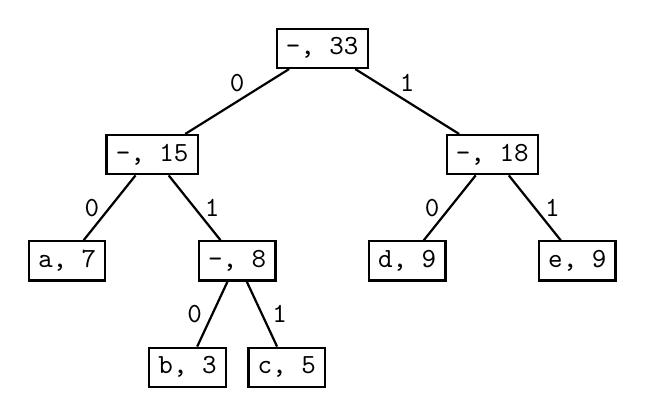
\begin{tikzpicture}
            [
                level distance=1.5cm,
                level 1/.style={sibling distance=4.8cm},
                level 2/.style={sibling distance=2.4cm},
                level 3/.style={sibling distance=1.4cm},
                thick,
                font=\ttfamily\bfseries, scale=0.9
            ]
            \tikzset{
                treenode/.style = {rectangle, draw=black, align=center,minimum width=0.75cm},
                edgestyleL/.style = {midway,left,draw=none},
                edgestyleR/.style = {midway,right,draw=none}
            }
            \node [treenode] (T) {-, 33}
            child { node[treenode] (L) {-, 15}
                    child { node[treenode] (LL) {a, 7} edge from parent node[edgestyleL] {0} }
                    child { node[treenode] (LR) {-, 8}
                            child { node[treenode] (LRL) {b, 3} edge from parent node[edgestyleL] {0} }
                            child { node[treenode] (LRR) {c, 5} edge from parent node[edgestyleR] {1} }
                            edge from parent node[edgestyleR] {1}
                        }
                    edge from parent node[edgestyleL,above] {0}
                }
            child { node[treenode] (R) {-, 18}
                    child { node[treenode] {d, 9} edge from parent node[edgestyleL] {0}}
                    child { node[treenode] {e, 9} edge from parent node[edgestyleR] {1}}
                    edge from parent node[edgestyleR,above] {1}
                }
            ;
        \end{tikzpicture}
        \caption{An example of Huffman tree.}
        \label{fig:tree}
    \end{figure}

\end{center}

\subsection{Decoding}
Once having the encoded file and the Huffman tree, it is straightforward to decompress the file to its original shape. The prefix alphabet ensures to have that it is possible to visit the tree using a DFS approach and get a unique decoded version of the file using an approach similar to \cref{alg:encode}.

\section{Parallel Huffman Implementation}
To parallelize our algorithm over threads and processes, we decided to follow this structure
\begin{itemize}
    \item multiple processes to process groups of file and folders separately;
    \item multiple threads to process different chunk of the same file in parallel.
\end{itemize}

There are a few motivations to our choice. Mainly are:

\begin{itemize}
	\item In most operating systems a file is a resource that the OS gives to a single process. We wanted to follow a similar design philosphy.
	\item Most operating system can allow multiple processes to open the same file in reading mode, but few allow to multiple processes to open the same file in writing mode. This is because that leads to potentially concurrency and data integrity issues.
	\item Because threads of the same process share the address space, we can avoid the expensive data transfer across processes by parallelizing a single file using threads instead of processes. 
\end{itemize}

The parallel algorithm follows the same exact procedure as a serial version.

However we decided to process a file using multiple threads.

That means that a single file is divided in chunks of a fixed size. 

Then the program forks the number of threads we intented.

One of them reads a number of chunks equal to the number of threads. When it's done reading the chunks, all threads can work on the processing.

Every chunk is processed by a single thread. 

When all threads are done processing their chunks, a thread writes the completed chunks to file. Because all threads share a memory space there is no need to perform data transfer.


The procedure is the same in both encoding and decoding. Also counting occurences follow a similar architectures, but without the write operations.





For multiple files, the rank 0 crawls all the files in the input directory. Then it opens all the files and reads their size. Then it creates a priorityQ where each item is a process and it inserts files in the priorityQ and updates the priority with the file size. This way we can ensure a proper almost equal work division among different processes.

When all this is done, the rank 0 sends the list of files to each process and then each process starts to work indipendetly on it's own list of files.


Implementation and detailed notes

We found that a size of 4096 bytes had  the best IO times, probably due to the fact that 4096B is the size of a page in most Linux based operating systems. The last chunk may be smaller.

We tried to parallelize the IO, having multiple threads that read it's own chunk. We found that the standard File Descriptor provided by C language has a lock to guarantee thread safety. However that slows down the reads significantly. Instead we tried using multiple file descriptors to circumvent this limitation. However we found no improvement over a serial read done by one thread for all the threads in it's team. This is likely because the OS schedules the IO requests and serves them one at the time, resulting in impossible truly parallel IO.

We also tested a architecture where we had two dedicated threads to IO, one for reading and one for writing chunks. This way the idea was that whenever a chunk was processed, the IO thread would read and write the related chunks, without delays due to the IO, and synchronizing the IO with locks to prevent inconstenstencies. However we found that this approach was a waste  of resources, as the IO on the cluster is extremely fast (5GB+/s) and would result in the IO threads being idle most of the time.

The schema is presented in Figure here

\section{Conclusions}
To conclude.


\bibliography{bibliography.bib}{}
\bibliographystyle{IEEEtran}

\end{document}
